\subsection{MixColumns transformation}

MixColumns transformation is most efficient to be implemented directly in $GF(2^8)$. Unlike in SubBytes transformation, all attempts to decompose operations lead to increase of overall number of required logic gates. This is because \cite{vlsi}:

\begin{itemize}[nolistsep]
\item mapping values to and from composite fields requires additional logic
\item constants used in MixColumns have less non-zero bits in $GF(2^8)$ ($\{02\}_{16}$, $\{03\}_{16}$) than in $GF((2^2)^4)$ ($\{5f\}_{16}$, $\{5e\}_{16}$), which results in more logic gates required to perform multiplication by them.
\end{itemize}

MixColumns transformation can be efficiently implemented by taking advantage of substructure sharing. Lets first notice that multiplying any $a \in GF(2^8)$ by $\{03\}_{16}$ can be substituted by multiplication by $\{02\}_{16}$ and one addition:

\begin{equation}
\label{eq:decomp_mul_3}
\{03\}_{16}a = (x + 1)a = ax + a = \{02\}_{16}a + a
\end{equation}

Taking that into consideration we can derive equations for MixColums transformation:

\begin{equation}
\label{xd}
\begin{aligned}
B_0' &= \{02\}_{16}B_0 + \{03\}_{16}B_1 + B_2 + B_3 \\
&\stackrel{(\ref{eq:decomp_mul_3})}{=}
\{02\}_{16}B_0 + (\{02\}_{16}B_1 + B_1) + B_2 + B_3 \\
&= \{02\}_{16}(B_0 + B_1) + (B_2 + B_3) + B_1 \\ \\
%
B_1' &= B_0 + \{02\}_{16}B_1 + \{03\}_{16}B_2 +  B_3 \\ 
&\stackrel{(\ref{eq:decomp_mul_3})}{=}
B_0 + (\{02\}_{16}B_1 + B_1) + \{02\}_{16}B_2 + B_3 \\ 
&= \{02\}_{16}(B_1 + B_2) + (B_0 + B_3) + B_2\\ \\
%
B_2' &= B_0 + B_1 + \{02\}_{16}B_2 + \{03\}_{16}B_3 \\
&\stackrel{(\ref{eq:decomp_mul_3})}{=}
B_0 + B_1 + \{02\}_{16}B_2 + (\{02\}_{16}B_3 + B_3) \\
&= \{02\}_{16}(B_2 + B_3) + (B_0 + B_1) + B_3 \\ \\
%
B_3' &= \{03\}_{16}B_0 + B_1 + B_2 + \{02\}_{16}B_3 \\
&\stackrel{(\ref{eq:decomp_mul_3})}{=}
(\{02\}_{16}B_0 + B_0) + B_1 + B_2 + \{02\}_{16}B_3 \\
&= \{02\}_{16}(B_0 + B_3) + (B_1 + B_2) + B_0
\end{aligned}
\end{equation}

where $B_i$ are AES bytes, $[B_0, B_1, B_2, B_3]$ is input column and $[B_0', B_1', B_2', B_3']$ is transformed column. MixColumns transformation for a single column can be therefore implemented as shown in figure \ref{fig:mix_columns}. MixColumns transformation on entire AES state consists of 4 such circuits.

\begin{figure}[!h]
\label{fig:mix_columns}

\centering
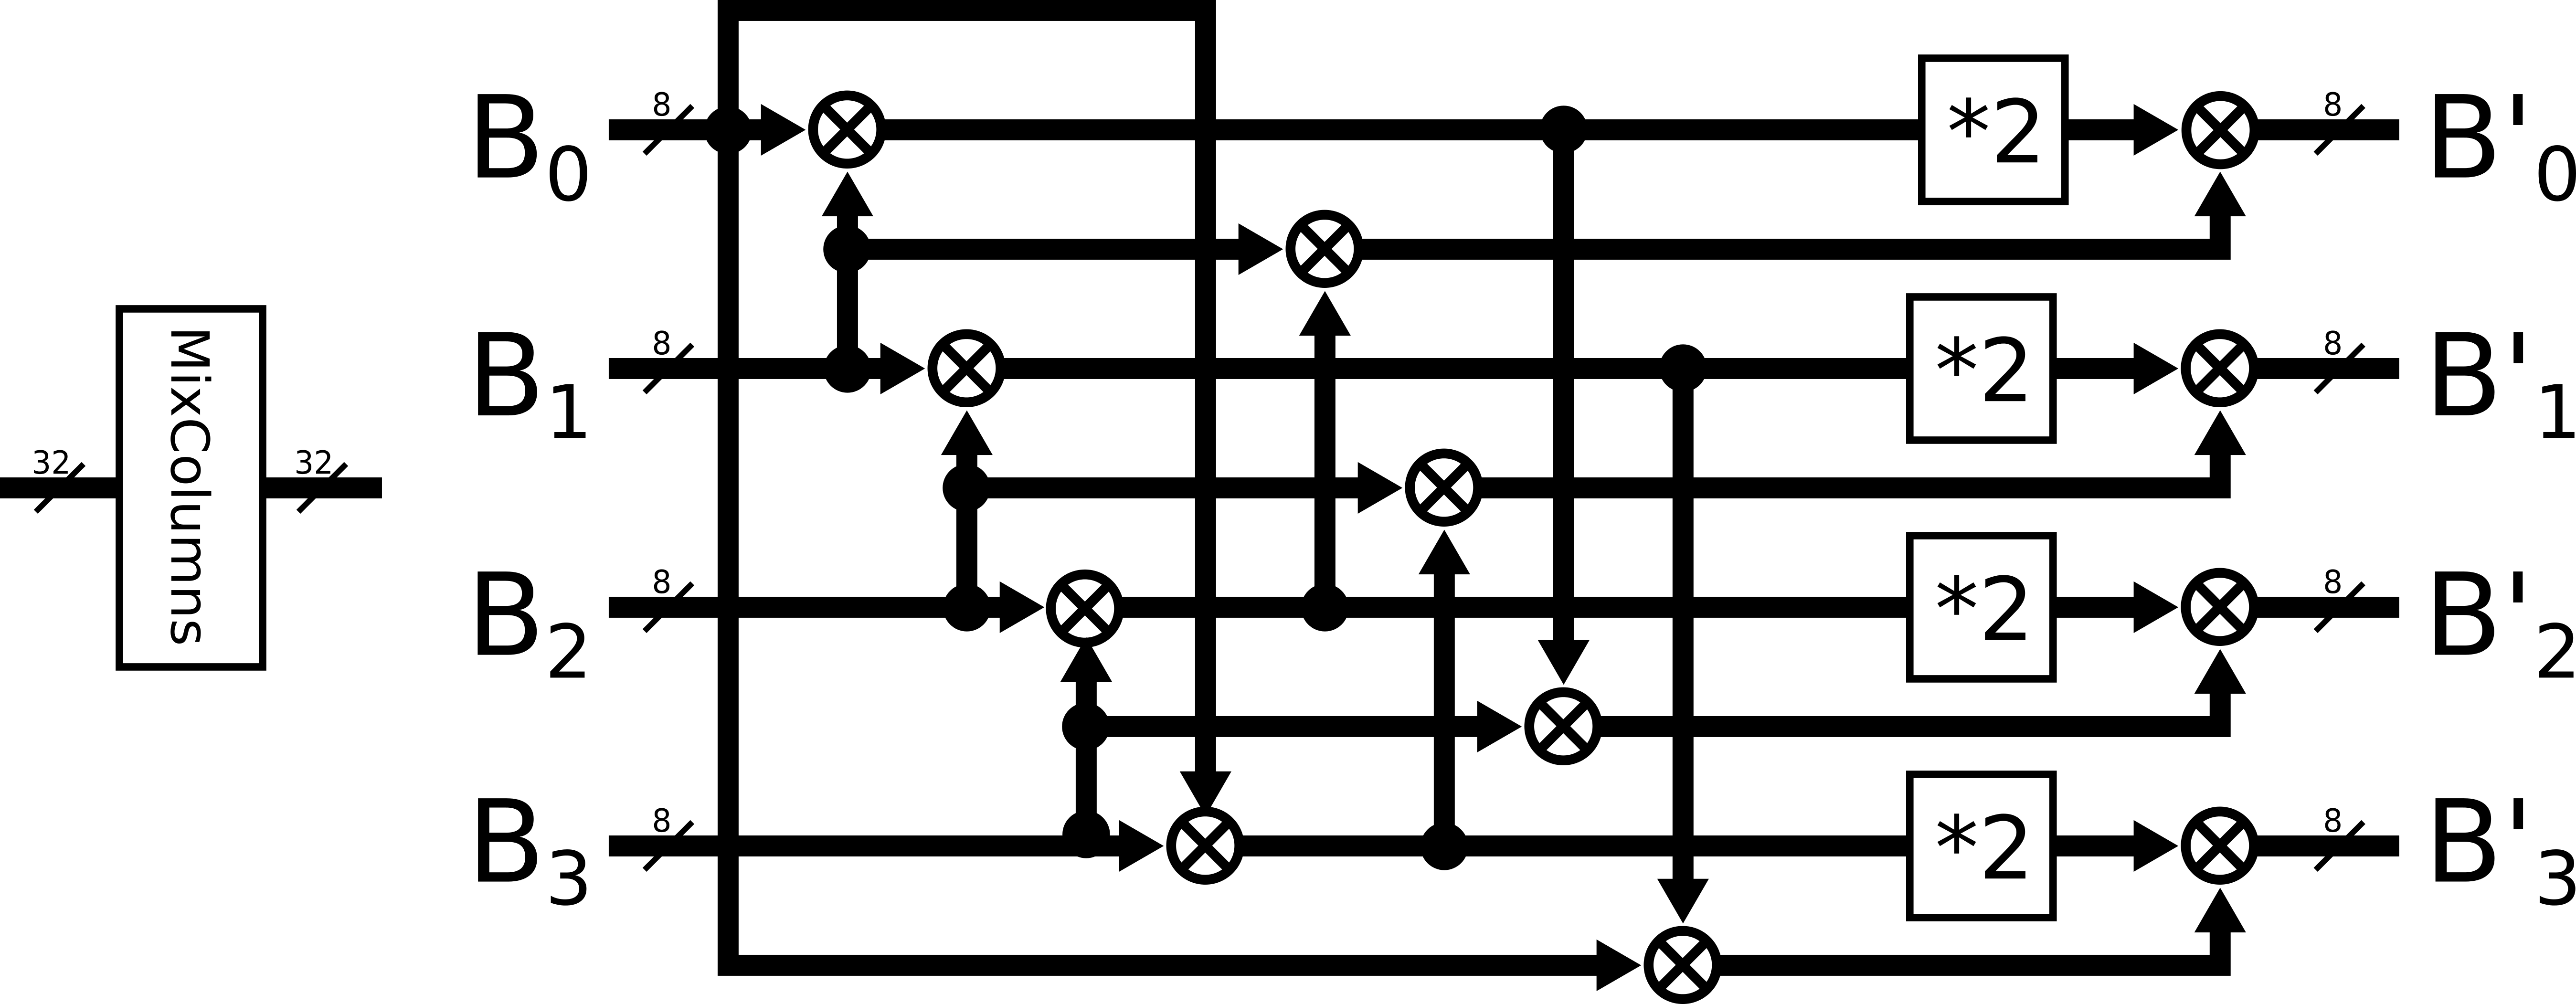
\includegraphics[scale=2.5]{mix-columns}

\caption{MixColumns transformation circuit}
\end{figure}

Multiplication by $\{02\}_{16}$ can be calculated according to formula (\ref{eq:mul2}) \cite{vlsi}: 

\begin{equation}
\label{eq:mul2}
\{02\}_{16}S = xS = s_6x^7 + s_5x^6 + s_4x^5 + (s_3 + s_7)x^4 + (s_2 + s_7)x^3 + s_1x^2 + (s_0 + s_7)x + s_7
\end{equation}

which requires 3 $xor$ gates.


